\documentclass[border=3pt]{standalone}
\usepackage{tikz}
\usetikzlibrary{decorations.pathreplacing,patterns}
\definecolor{greengreen}{rgb}{0.0, 0.42, 0.24}
%%%%%%%%%%%%%%%%%%%%%%%%%%%%%%%%%%%%%%%%%%%%%%%%%%%%%%%%%%%%%%%%%
\begin{document}
%%%%%%%%%%%%%%%%%%%%%%%%%%%%%%%%%%%%%%%%%%%%%%%%%%%%%%%%%%%%%%%%%
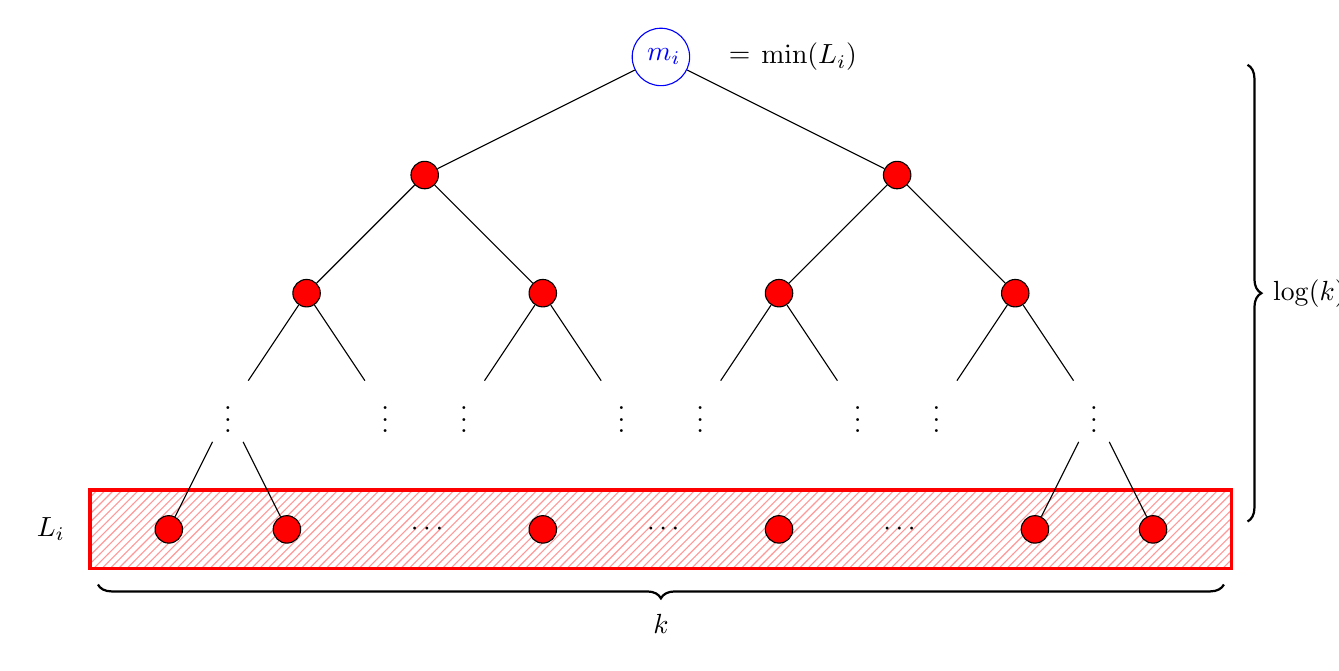
\begin{tikzpicture}[every node/.style={align=center},red/.style={fill=red,draw,circle,inner sep=0pt}, text width = .35cm]
%================================================================
%	Box
\draw[color=red,very thick, pattern=north east lines, pattern color=red!40] (-1,-0.5) rectangle (13.5,0.5);
%================================================================
%	Nodes
\node[style=red] (a1) at (0,0) {};
\node[style=red] (a2) at (1.5,0) {};
\node at (3.25,0) {$\cdots$};
\node[style=red] at (4.75,0) {};
\node at (6.25,0) {$\cdots$};
\node[style=red] at (7.75,0) {};
\node at (9.25,0) {$\cdots$};
\node[style=red] (a3) at (11,0) {};
\node[style=red] (a4) at (12.5,0) {};
%----------------------------------------------------------------
\node (b1) at (0.75,1.5) {$\vdots$};
\node (b2) at (2.75,1.5) {$\vdots$};
\node (b3) at (3.75,1.5) {$\vdots$};
\node (b4) at (5.75,1.5) {$\vdots$};
\node (b5) at (6.75,1.5) {$\vdots$};
\node (b6) at (8.75,1.5) {$\vdots$};
\node (b7) at (9.75,1.5) {$\vdots$};
\node (b8) at (11.75,1.5) {$\vdots$};
%----------------------------------------------------------------
\node[style=red] (c1) at (1.75,3) {};
\node[style=red] (c2) at (4.75,3) {};
\node[style=red] (c3) at (7.75,3) {};
\node[style=red] (c4) at (10.75,3) {};
%----------------------------------------------------------------
\node[style=red] (d1) at (3.25,4.5) {};
\node[style=red] (d2) at (9.25,4.5) {};
%----------------------------------------------------------------
\node[draw, circle, color = blue] (e1) at (6.25,6) {$m_i$};

%================================================================
%	Lines
\draw (a1) -- (b1);
\draw (a2) -- (b1);
\draw (a3) -- (b8);
\draw (a4) -- (b8);
%----------------------------------------------------------------
\draw (b1) -- (c1);
\draw (b2) -- (c1);
\draw (b3) -- (c2);
\draw (b4) -- (c2);
\draw (b5) -- (c3);
\draw (b6) -- (c3);
\draw (b7) -- (c4);
\draw (b8) -- (c4);
%----------------------------------------------------------------
\draw (c1) -- (d1);
\draw (c2) -- (d1);
\draw (c3) -- (d2);
\draw (c4) -- (d2);
%----------------------------------------------------------------
\draw (d1) -- (e1);
\draw (d2) -- (e1);

%================================================================
%	Decoration
\draw[thick, decorate,decoration={brace,amplitude=5pt,mirror}] (13.7,0.1) -- (13.7,5.9);
\draw[thick, decorate,decoration={brace,amplitude=5pt,mirror}] (-0.9,-0.7) -- (13.4,-0.7);
%----------------------------------------------------------------
\node at (14.2,3) {$\log(k)$};
\node at (-1.5,0) {$L_i$};
\node at (6.25,-1.2) {$k$};
\node at (7.7,6) {$\min(L_i)$};
\node at (7.25,6) {$=$};
\draw[color=white] (14.5,0) -- (14.5,0.01);
%================================================================
\end{tikzpicture}
%%%%%%%%%%%%%%%%%%%%%%%%%%%%%%%%%%%%%%%%%%%%%%%%%%%%%%%%%%%%%%%%%
\end{document}
%%%%%%%%%%%%%%%%%%%%%%%%%%%%%%%%%%%%%%%%%%%%%%%%%%%%%%%%%%%%%%%%%